\section{Test}
Tutti i test sono stati eseguiti su una macchina con sistema operativo windows 10, un processore Intel Core i7 4750HQ a 2.0GHz e con 12Gb di RAM DDR3, e settando la maxThreshold a 5, con Approx spuntato e senza nessun parametro.\\
Per ogni dataset utilizzato abbiamo testato l'algoritmo tramite la classe \textbf{Domino.java} descritto nel capitolo di implementazione, ricavando così i tempi impiegati su ciascun dataset, provando ogni possibile colonna come RHS e le restanti colonne come LHS.  \\

Mostreremo quelli che sono i test ritenuti rilevanti:
\begin{itemize}
	\item Test in sequenziale con \textbf{FixedThreadPoo};
	\item Test in parallelo con \textbf{CachedTreadPool};
\end{itemize}
\subsection{Dataset utilizzati}
Oltre ad una serie di dataset creati appositamente per verificare la correttezza di alcune operazioni, abbiamo prelevato una serie di dataset dal sito dell'Information Systems Group dell'Hasso-Plattner-Institut \cite{metanome}: un un gruppo di ricerca della suddetta Università tedesca che si occupa, tra le altre cose, di progettare algoritmi dedicati alla ricerca delle dipendenze funzionali. Su tale sito, oltre a poter consultare gli algoritmi sviluppati, è possibile accedere a tutti i dataset sui quali tali algoritmi sono stati testati corredati a varie informazioni (i.e. fonte, numeri di attributi, numero di righe, dipendenze funzionali trovate, dipendenze funzionali ordinate trovate ecc).\\
\begin{table}[H]
	\centering
	\begin{tabular}{|c|c|c|c|}
		\hline 
		\textbf{Dataset} & \textbf{Colonne} & \textbf{Righe}  & \textbf{Size [KB]} \\ 
		\hline 
		Foodstamp.csv & 4  & 150 & 3 \\ 
		\hline 
		Emissions.csv& 4 & 8088 &479  \\ 
		\hline 
		Vocab.csv& 4 & 21638 &530  \\ 
		\hline 
		Iris.csv& 5 &  150&5  \\ 
		\hline 
		Car.csv&7  &  1728&51  \\ 
		\hline 
		Chess.csv&7  &28056  &519  \\ 
		\hline 
		Breast-Cancer.csv& 11 & 699  & 20  \\ 
		\hline 
		Bridges.csv& 13 & 108 &  6\\ 
		\hline 
		Echocardiogram.csv& 13 & 132 & 6 \\ 
		\hline 
	\end{tabular}
	\caption{Dataset utilizzati}
	\label{tab:Dataset utilizzati}
\end{table}

\subsection{Tempi}
	In questa fase di testing mostreremo i risultati ottenuti lavorando in sequenziale e parallelo. Nella seguente tabella sono mostrati i risultati ottenuti dai test sui
dataset considerati, considerando come unità di tempo i minuti.
\begin{table}[H]
\resizebox{\textwidth}{!}{
	\begin{tabular}{|c|c|c|c|c|c|c|}
		\hline 
		\textbf{Dataset} & \textbf{Seq. Threshol 5} & \textbf{Par. Threshol 5} & \textbf{Seq. Approx} &\textbf{Par. Approx} & \textbf{Seq. Nessun Parametro} & \textbf{Par. Nessun Parametro} \\ 
		\hline 
		Foodstamp.csv & 0,02033333  & 0,02053333 &0,02068333 &0,02041667 &0,02168333 &0,02133333\\ 
		\hline 
		Emissions.csv& 0,46033333 & 0,45738333 &0,49261667 &0,52401667 &0,86556667 &1,1295  \\ 
		\hline 
		Vocab.csv& 4,42098333 & 4,25195 &4,34378333 &4,33988333 &4,28013333 &5,37476667 \\ 
		\hline 
		Iris.csv& 0,03138333 & 0,0314 &0,01945 &0,01951667 &0,01986667 &0,01845 \\ 
		\hline 
		Car.csv&0,1217333  & 0,11505 &0,07536667 &0,09918333 &0,09873333 &0,07543333\\ 
		\hline 
		Chess.csv&38,80671667  &25,53381667  &8,68918333 &8,38323333 &8,5204 &8,45833333  \\ 
		\hline 
		Breast-Cancer.csv& 31,90678333 & 25,53381667  &1,4976 &0,87755 &1,3184167 & 0,87385 \\ 
		\hline 
		Bridges.csv& 6,29508333 & 4,15786667  &5,88285 &5,73366667 &16,93371667 &13,1462667\\ 
		\hline 
		Echocardiogram.csv& 12,6269167 & 9,50878333 &4,94633333 &4,92563333 &6,78765 & 4,92665\\ 
		\hline 
	\end{tabular}
}
	\caption{Tempi}
	\label{tab:Tabella Tempi}
\end{table}

	Di Seguito mostriamo il grafico relativo alla \ref{tab:Tabella Tempi}
\begin{figure}[H]
	\centering
	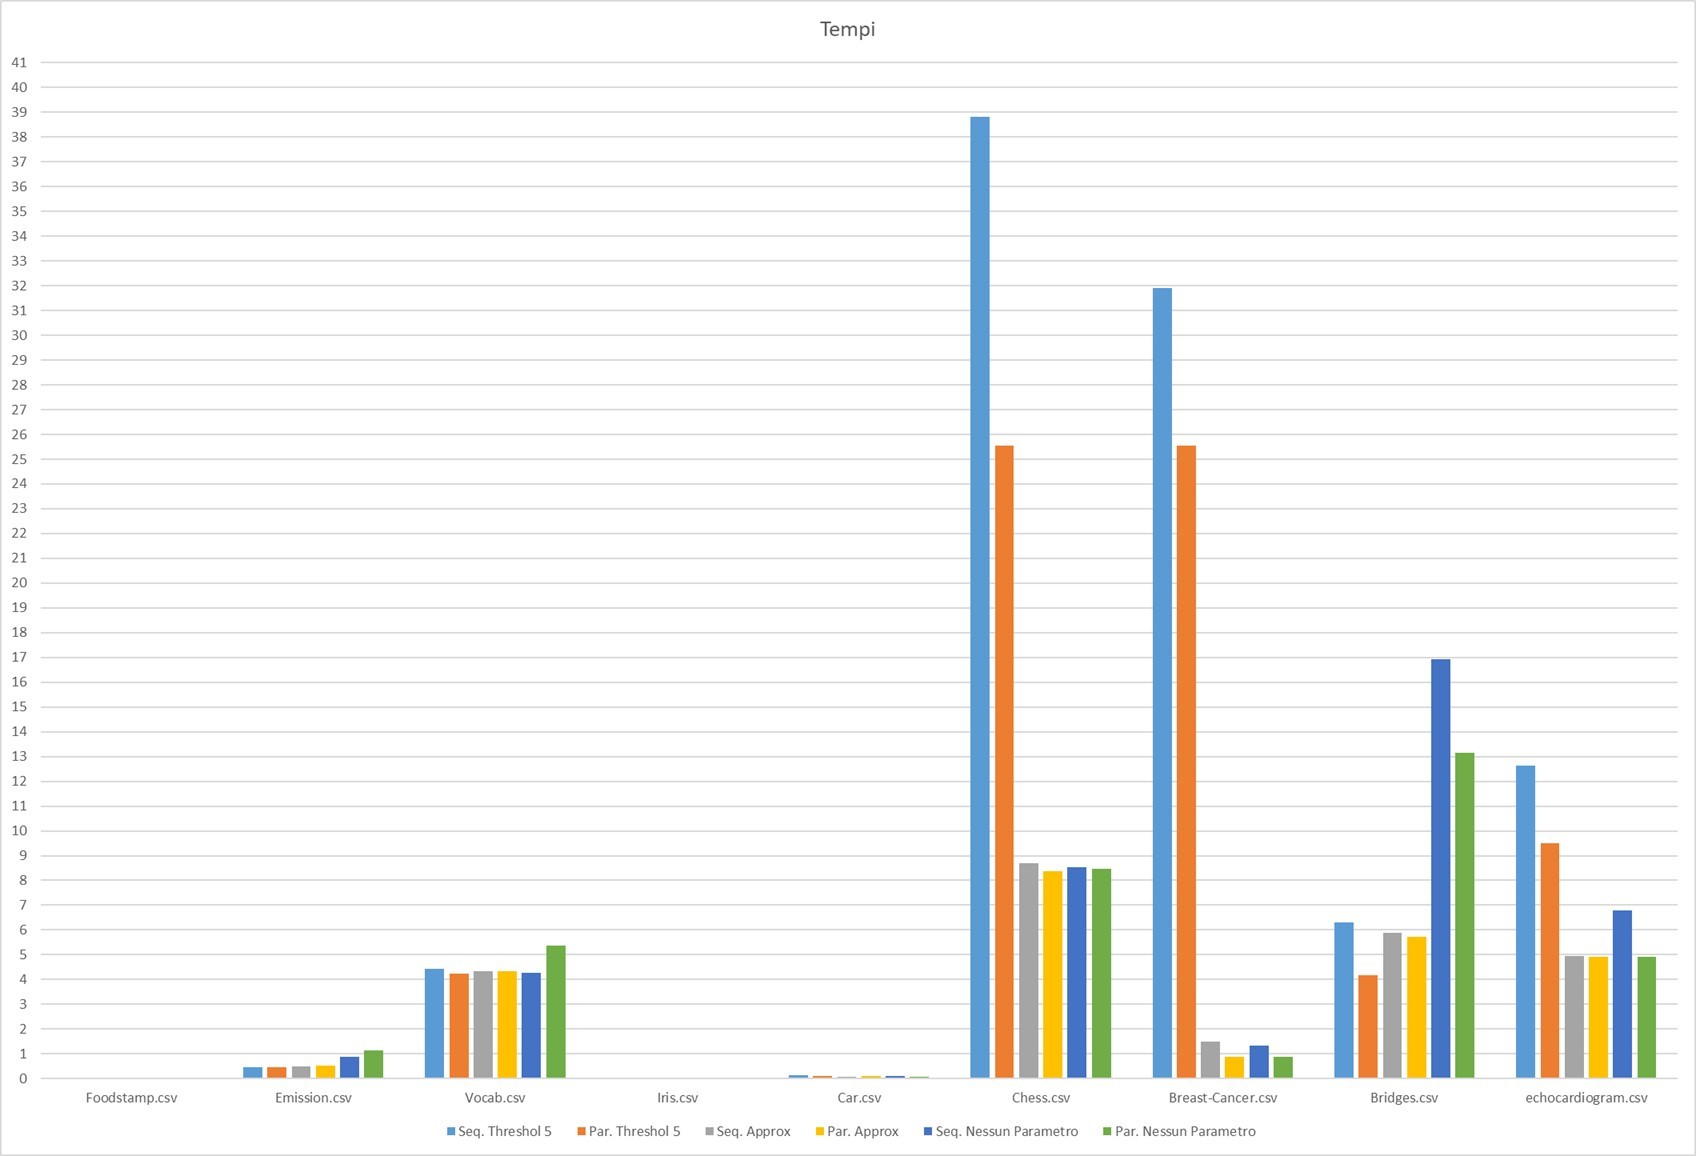
\includegraphics[scale=0.43]{Immagini/GraficoTempi.jpg}
	\caption{Grafico Tempi}
	\label{fig:Grafico Tempi}
\end{figure}

\subsection{Miglioramenti}
	In questa fase mostreremo i miglioramenti ottenuti passando dal sequenziale al parallelo. Nella seguente tabella sono mostrati i risultati ottenuti dai test sui dataset considerati in forma percentuale.

	\begin{table}[H]
		\resizebox{\textwidth}{!}{
			\begin{tabular}{|c|c|c|c|}
				\hline 
				\textbf{Dataset} & \textbf{Percentuale miglioramento Threshold 5} & \textbf{Percentuale miglioramento Approx} & \textbf{Percentuale miglioramento Nessun Parametro} \\ 
				\hline 
				Foodstamp.csv & -0,983606719  &1,289250812 &1,614143215\\ 
				\hline 
				Emissions.csv& 0,640839976 & -6,37412453 &-30,49254773  \\ 
				\hline 
				Vocab.csv& 3,823432874 & 0,089783484 &-25,57474863 \\ 
				\hline 
				Iris.csv& -0,053117372 & -0,34277635 &7,130888065  \\ 
				\hline 
				Car.csv&5,490116509  & -31,60105123 &23,59892045\\ 
				\hline 
				Chess.csv&34,20258434  &3,52104436567  &0,728447843   \\ 
				\hline 
				Breast-Cancer.csv& 19,97370463 & 41,40291132  &33,71974126  \\ 
				\hline 
				Bridges.csv& 33,9505698 & 2,535902326  &22,3663242 \\ 
				\hline 
				Echocardiogram.csv& 24,69433706 & 0,418491812 &27,41744197 \\ 
				\hline 
			\end{tabular}
		}
		\caption{Miglioramenti}
		\label{tab:Tabella Miglioramenti}
	\end{table}
Di Seguito mostriamo il grafico relativo alla \ref{tab:Tabella Miglioramenti}

\begin{figure}[H]
	\centering
	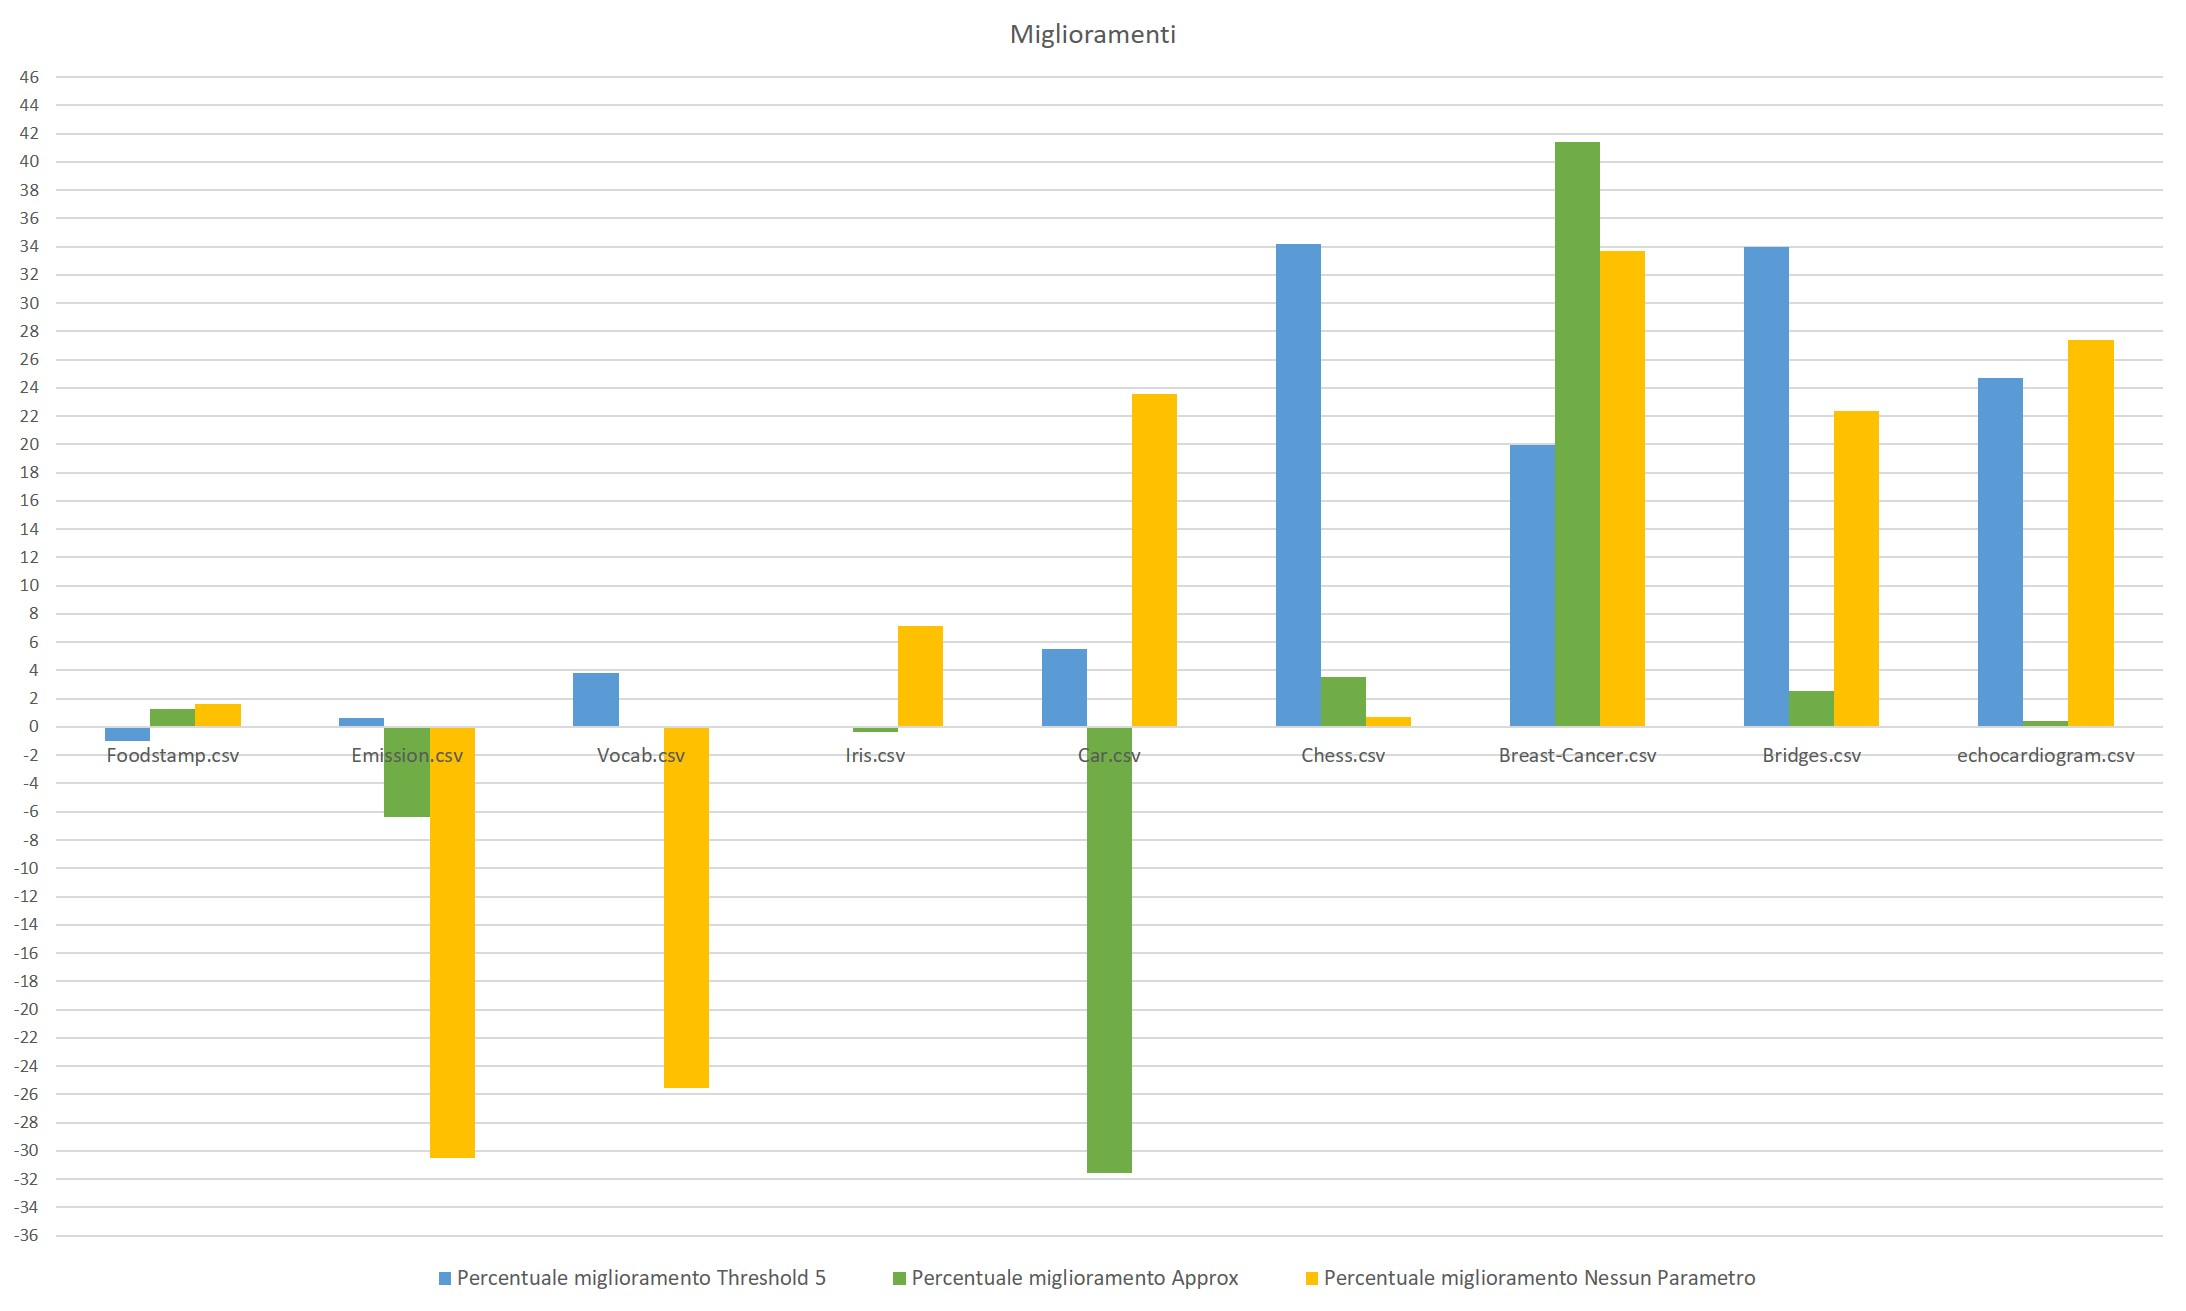
\includegraphics[scale=0.43]{Immagini/GraficoMiglioramenti.jpg}
	\caption{Grafico Miglioramenti}
	\label{fig:Grafico Miglioramenti}
\end{figure}

\section{Conclusioni}
Dopo aver completato la descrizione del progetto sviluppato è necessario fare qualche osservazione:  dalla tabella \ref{tab:Tabella Miglioramenti} possiamo notare che alcuni dataset presentano un peggioramento in termini di prestazioni. Questi risultati sono dovuti dal fatto che l'ammontare di computazione di alcuni dataset era minore dei tempi di sincronizzazione e ricombinazione dei thread generati.
\section{Lavori Futuri}
Durante la fase di testing, si è notato che la parte che prendeva più tempo era la parte di MinimalityAndGeneration; su di essa è stata effettuata una parallelizzazione a grana grossa ma, per ottenere prestazioni migliori, è possibile eseguire una parallelizzazione a grana fine.
